\chapter{Chương Trình Minh Họa}
\label{chap:presentation}

%==================================================================
\section{Mô hình chương trình}
Chương trình minh họa được cài đặt trên môi trường ứng dụng WEB sử dụng các công nghệ \textbf{Servlet, Bootstrap, Javascript AngularJS}.
%--------------------------------------------------------------
\subsection{Tổng Quan}
\begin{figure}
	\centering
	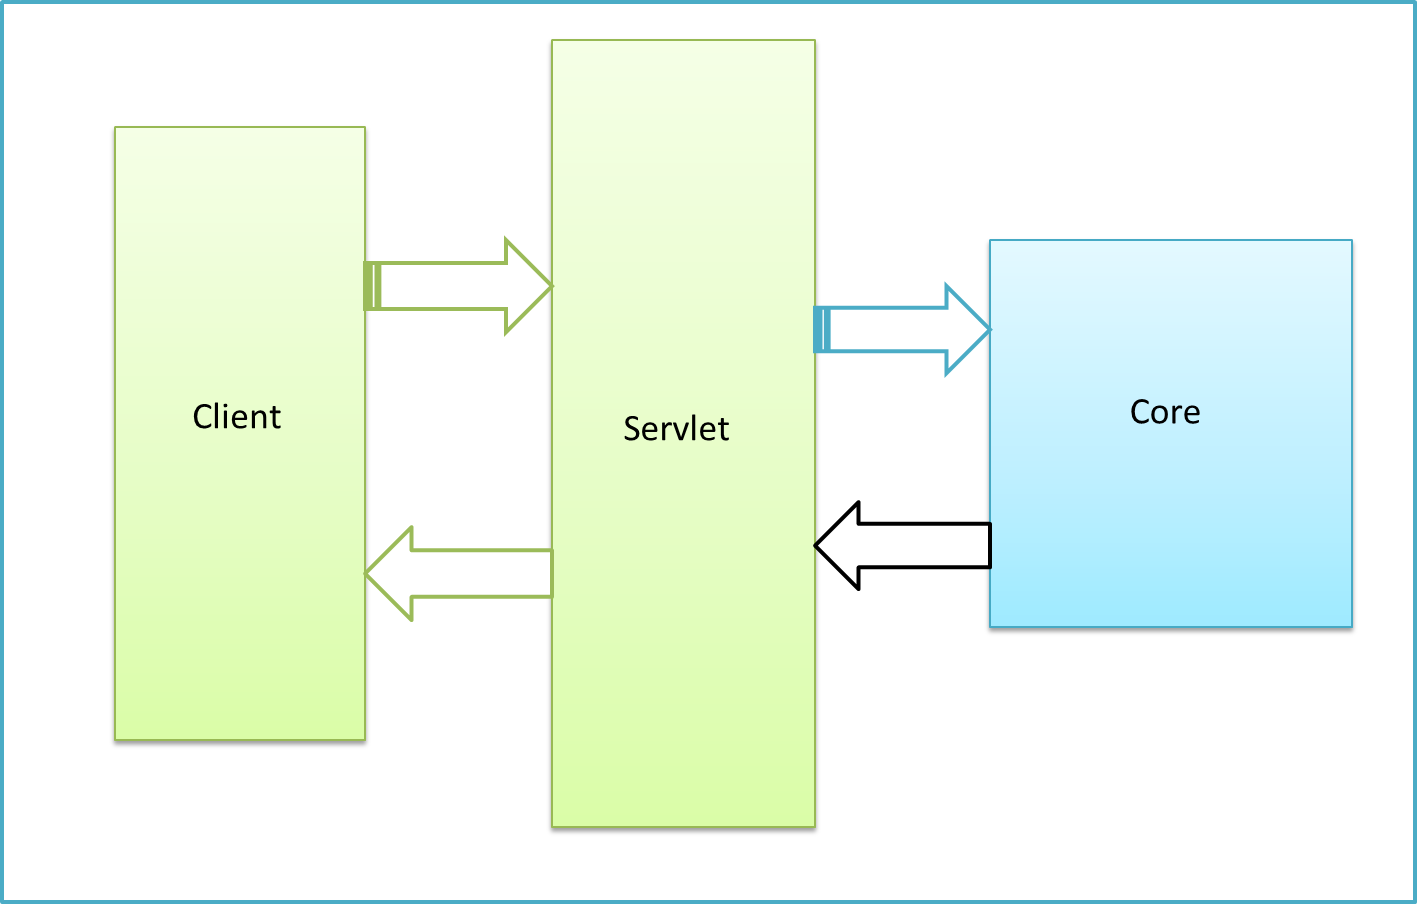
\includegraphics[scale=0.5]{figures/app-overview.png}
	\caption{Kiến trúc tổng quan ứng dụng \label{fig:appOverview}}
\end{figure}

Hình \ref{fig:appOverview} mô tả kiến trúc tổng quan của ứng dụng web cho bài toán đóng thùng 2D, chương trình gồm 3 phần:
\begin{itemize}
	\item \textbf{Core} chứa các lớp xử lý nghiệp vụ của bài toán đóng thùng, bao gồm đọc ghi dữ liệu, mô hình hóa và thực hiện tìm kiếm.
	\item \textbf{Servlet} chứa các lớp xử lý yêu cầu từ phía trình duyệt web của người dùng, nó xử lý các thao tác điều khiển của người dùng và cũng là nơi trả lại các thông tin cần thiết về cho client.
	\item \textbf{Client} là ứng dụng ở phía người dùng xử lý các thông tin trả về từ servlet và hiển trị lên màn hình trình duyệt web.
\end{itemize}
Cụ thể các phần của chương trình như sau:
%--------------------------------------------------------------
\subsection{Server}
\subsubsection{Core}
Phần \textbf{Core} bao gồm:
\begin{itemize}
	\item Các lớp xử lý việc đọc dữ liệu từ hệ thống tệp tin của Server, các lớp này nằm trong gói \textit{binpacking.io}
	\begin{itemize}
		\item \textsf{BpData} chứa các thông tin của tệp tin dữ liệu, mỗi đối tượng của lớp này chứa đầy đủ thông tin của một tệp tin dữ liệu của BP2D: tệp tin (\textit{file}), chiều rộng thùng (\textit{binWidth}), chiều cao thùng (\textit{binHeight}), số lượng vật phẩm (\textit{itemCount}), chiều rộng các vật phẩm (\textit{itemHeights}), chiều cao các vậy phẩm (\textit{itemHeights}). Ngoài ra các đối tượng của lớp này chỉ thực sự đọc dữ liệu khi cần thiết, điều này giúp cải thiện hiệu năng hệ thống, tiết kiệm tài nguyên máy chủ.
		\begin{lstlisting}
		//BpData.java
		
		private File file;
		private boolean isReady;
		private int binWidth;
		private int binHeight;
		private int itemCount;
	
		private int[] itemWidths;
		private int[] itemHeights;
		
		\end{lstlisting}
		\item \textsc{BpDataManager} quản lý toàn bộ các đối tượng \textsf{BpData}, bảo đảm mỗi đối tượng \textsf{BpData} luôn chỉ cần khởi tạo một lần và có thể sử dụng cho nhiều mô hình khác nhau. Đối tượng của lớp này sẽ là nơi cung cấp dữ liệu cho các lớp yêu cầu xử lý mô hình, tìm kiếm\dots.
	\end{itemize}
	\item Lớp mô hình hóa cho bài toán \textsf{BpModelCombine} nằm trong gói \textit{binpacking2d.model} có tác dụng mô hình bài toán đóng thùng vào thư viện JOpenCBLS.
	\item Các lớp khởi tạo phương án bắt đầu cho bài toán, mỗi lớp khởi tạo sẽ có một cách thức khởi tạo riêng cho các mô hình tương ứng. Với bài toán BP2D có các cách khởi tạo tương ứng với các lớp:
	\begin{itemize}
		\item \textsf{BpAllZeroInitMethod} khởi tạo phương án bằng cách xếp tất cả các vật phẩm vào vị trí góc của thùng và không có vật phẩm nào được xoay.
		\item \textsf{BpRandomInitMethod} khởi tạo một cách ngẫu nhiên vị trí các vật phẩm, chúng cũng có thể được xoay hoặc không và hoàn toàn ngẫu nhiên.
	\end{itemize}
	Ngoài ra các đối tượng của các lớp khởi tạo này cũng được quản lý bởi đối tượng của lớp \textsf{BpInitMethodManager}, đối tượng này sẽ chỉ cho hệ thống những lớp khởi tạo nào được phép sử dụng và khởi tạo sẵn các lớp khởi tạo.
	\item Chương trình còn cài đặt thêm một số lớp có chức năng tương tự như trong thư viện JOpenCBLS có tác dụng thử nghiệm và phù hợp hơn với chương trình đa luồng.
\end{itemize}

\subsubsection{Servlet}
Các Servlet là các lớp nằm trong gói \textit{binpacking2d.servlet} có vai trò giao tiếp với client, bao gồm:
\begin{itemize}
	\item \textbf{control - ControlServlet} là Servlet chịu trách nhiệm nhận các thông điệp điều khiển từ phía người dùng sau đó nó tương tác với phần Core để thực hiện các tác vụ này. \textsf{ControlServlet} xử lý các thông điệp từ các phương thức GET của http:
	\begin{itemize}
		\item \textit{control?action=init{\&}initMode=<modeId>{\&}fileId=<fileId>} khởi tạo mô hình bằng chỉ số của thủ tục tìm kiếm và chỉ số của tệp tin trên hệ thống, các chỉ số định danh này được cố định và được cung cấp bởi các quản lý tương ứng: \textsc{SearchMethodManager, BpDataManager}.
		\item \textit{control?action=start} bắt đầu tiến trình tìm kiếm cục bộ đã được khởi tạo trước đó, nếu chưa được khởi tạo trước thì thao tác này sẽ không thực hiện tìm kiếm.
		\item \textit{action=stop} sẽ dừng tiến trình tìm kiếm đang thực thi trên máy chủ.
	\end{itemize}
	\item \textbf{events - EventsServlet} sẽ liệt kê tất cả các sự kiện diễn ra trên máy chủ trong quá trình tìm kiếm, các sự kiện được trả dưới dạng JSON cấu trúc như sau: 
		\begin{lstlisting}
		{
			"state": {
				"running": RUNNING_VALUE,
				"ready": READY_VALUE
			}
			"events":[
				{
					"violations": VIOLATION,
					"name": EVENT_NAME,
					"items": LIST_ITEMS
				},
				...
			]
		}
		\end{lstlisting}
	
	\item \textbf{fetch - ResourceServlet} là Servlet chịu trách nhiệm xử lý các yêu cầu lấy thông tin tài nguyên từ người dùng, nó cung cấp các loại tài nguyên:
	\begin{itemize}
		\item \textit{fetch?res=files} khi nhận được yêu cầu này nó sẽ trả về dưới dạng JSON các tệp tin dữ liệu của bài toán BP2D đang có trên thư mục dữ liệu của máy chủ. Thông điệp trả về sẽ có dạng JSON:
		\begin{lstlisting}
		[
			{		
				"name": FILE_NAME,
				"id" : FILE_ID
			},
			...
		]
		\end{lstlisting}
		\item \textit{fetch?res=search} cung cấp các thuật toán tìm kiếm đã được cài đặt trong ứng dụng của máy chủ, thông tin trả về dưới dạng JSON:
		\begin{lstlisting}
		[
			SEARCH_METHOD,
			...
		]
		\end{lstlisting}
		\item \textit{fetch?res=init} cung cấp các thuật toán khởi tạo dưới dạng JSON:
		\begin{lstlisting}
		[
			INIT_METHOD,
			...
		]
		\end{lstlisting}
	\end{itemize}
\end{itemize}

%--------------------------------------------------------------
\subsection{Client}
Chương trình phía client được cài đặt sử dụng công nghệ AngularJS và Bootstrap:
\begin{itemize}
	\item \textsc{AngularJS} là một framework javascript được phát triển bởi các kỹ sư của Google, nó thay đổi cách các lập trình viên làm việc với javascript, cung cấp các cách thức lập trình nhanh, logic, hiệu quả trên các ứng dụng web.
	\item \textsc{Bootstrap3} là một thư viện css3 nhằm làm cho việc thiết kế các trang web trở nên đơn giản, chuẩn mực.
\end{itemize}

Trong ứng dụng phía client của bài toán BP2D sử dụng các thành phần:
\begin{itemize}
	\item \textit{bin.js} định nghĩa chỉ thị của AngularJS, khi nó được khai báo trên html canvas, nó sẽ vẽ ra hình ảnh để mô tả vị trí của các vật phẩm trong thùng, nếu các vật chồng lấn lên nhau nó sẽ thông báo bằng cách vẽ viền của nó màu đỏ.
	\item \textit{poller.js} khai báo một dịch vụ mới trên AngularJS, dịch vụ này được AngularJS thực thi khi khởi tạo và nó được thực thi trong suốt quá trình ứng dụng phía client được mở. Khi được hoạt động, nó sẽ định kỳ lấy các sự kiện từ trên máy chủ về và dùng các hàm xử lý được khai báo trước để xử lý các dữ liệu sự kiện này. Thông thường các hàm xử lý sẽ cập nhật hiển thị các vật nằm trong thùng.
	\item \textit{index.js} định nghĩa ứng dụng AngularJS, thiết lập các hàm xử lý sự kiện cho \textit{poller} và thực hiện các thao tác khởi tạo cần thiết.
	\item \textit{index.html} là trang html chính của ứng dụng BP2D, nó GET từ Server và được cập nhật liên tục khi các sự kiện xảy ra.
\end{itemize}
%--------------------------------------------------------------
\subsection{Giao tiếp}
Khi máy chủ tiếp nhận một yêu cầu từ phía client, nó sẽ gửi về tệp tin \textit{index.html} cho client để thực thi trên trình duyệt web. Khi bắt đầu ứng dụng web phía client sẽ thực hiện lấy các thông tin tài nguyên từ máy chủ như các tệp tin, các thủ tục khởi tạo, các thuật toán tìm kiếm và đồng thời nó cũng yêu cầu máy chủ khởi tạo sẵn với một số tham số mặc định. Với ứng dụng web phía client này, người dùng có thể thực hiện các thao tác:
\begin{itemize}
	\item Lựa chọn tệp tin dữ liệu: ứng dụng cho phép người dùng lựa chọn tệp tin dữ liệu thông qua bảng chọn. Khi người dùng lựa chọn xong tệp tin dữ liệu, client sẽ yêu cầu server thực hiện luôn thao tác khởi tạo tương ứng.
	\item Lựa chọn thủ tục khởi tạo: khi người dùng thay đổi thủ tục khởi tạo chương trình cũng sẽ tự động gửi yêu cầu khởi tạo lên server và tự động cập nhật trạng thái lên màn hình.
	\item Lựa chọn thuật toán tìm kiếm: chương trình cung cấp nhiều lựa chọn tìm kiếm cho bài toán, các thuật toán được cài đặt một cách tổng quát và có thể dùng cho nhiều mô hình.
	\item Bắt đầu tìm kiếm: Người sử dụng được cung cấp một nút bấm để thực hiện tìm kiếm sau khi các thao tác khởi tạo được hoàn thành. Khi người sử dụng thực hiện thao tác này, client sẽ gửi một thông điệp điều khiển lên server yêu cầu bắt đầu thuật toán tìm kiếm.
	\item Kết thúc: Trong quá trình thực thi tìm kiếm, người sử dụng có thể dừng tiến trình này bằng cách bấm nút kết thúc, client sẽ gửi một thông điệp điều khiển kết thúc lên server và ngay lập tức server sẽ dừng công việc tìm kiếm.
\end{itemize}

Ngoài ra trong quá trình thực hiện tìm kiếm, client luôn luôn gửi các yêu cầu lấy danh sách sự kiện diễn ra trên server để cập nhật lên màn hình trình duyệt, các yêu cầu này được gửi một cách định kỳ.

%==================================================================
\section{Giao diện người dùng}
\subsection*{Khởi tạo dữ liệu}
\begin{figure}[H]
	\centering
	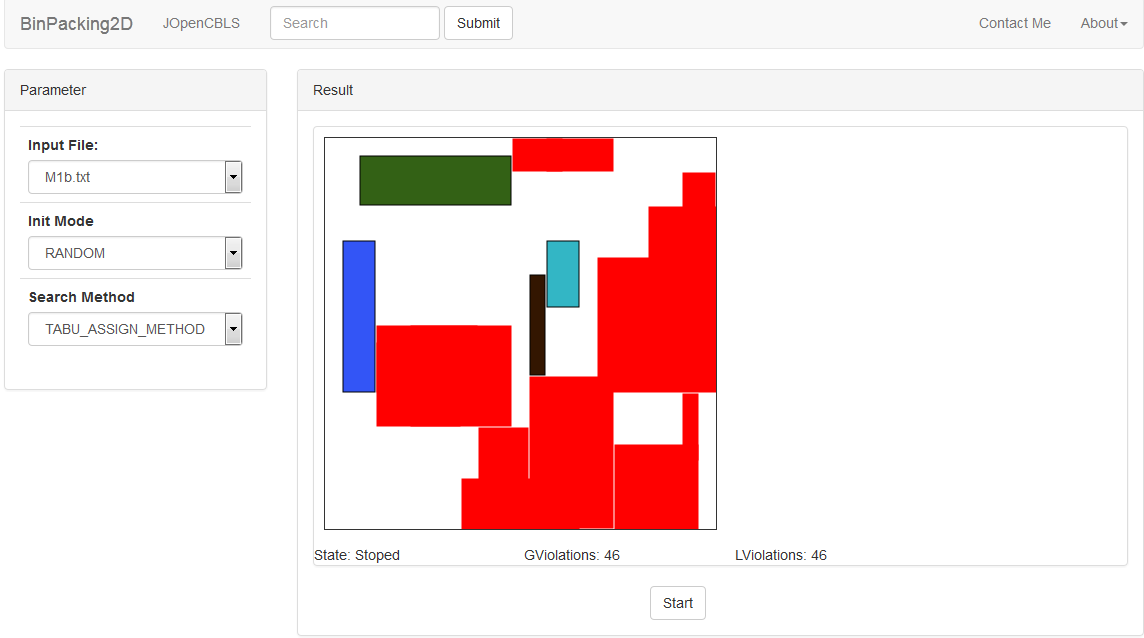
\includegraphics[scale=0.5]{figures/if-init.png}
	\caption{Giao diện khởi tạo chương trình \label{fig:ifInit}}
\end{figure}

Khi ứng dụng được khởi chạy, khi người dùng lựa chọn thay đổi bộ dữ liệu hoặc khi thay đổi thủ tục khởi tạo thì chương trình sẽ thực hiện khởi tạo mặc định các tham số và hiển thị lên màn hình như hình \ref{fig:ifInit}. Chương trình sẽ hiển thị các vật phẩm được xếp vào thùng không thỏa mãn các ràng buộc bởi màu đỏ, các vật thỏa mãn các ràng buộc sẽ được hiển thị bởi một màu nhẹ ngẫu nhiên.
\subsection*{Thực hiện tìm kiếm}
\begin{figure}
	\centering
	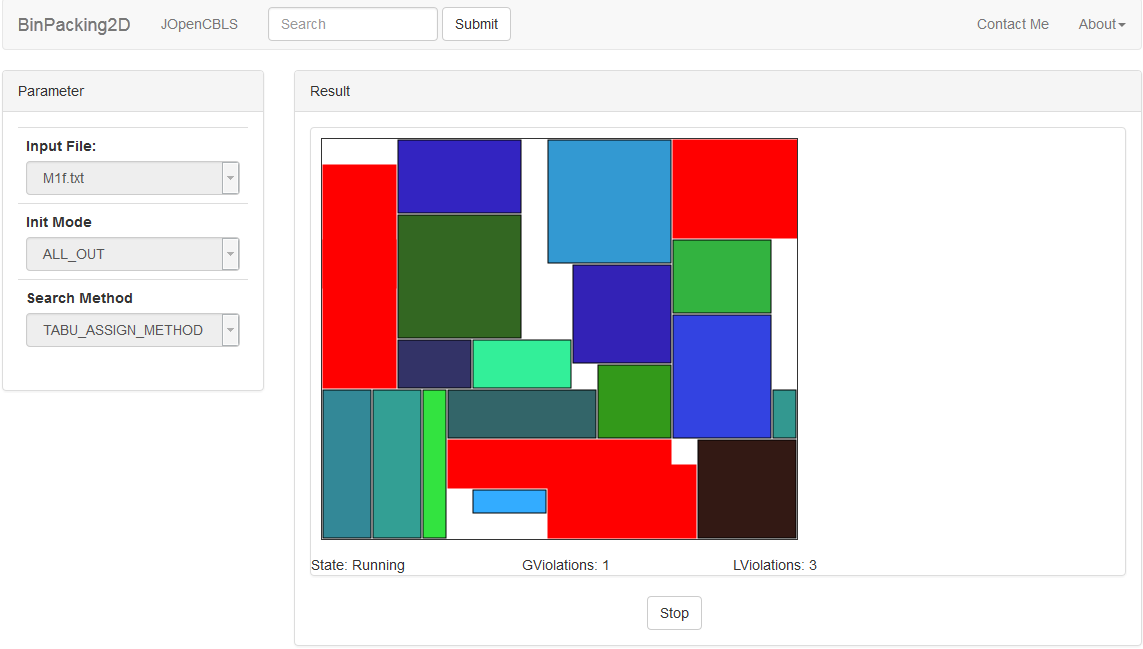
\includegraphics[scale=0.5]{figures/if-progress.png}
	\caption{Giao diện thực hiện tìm kiếm \label{fig:ifProgress}}
\end{figure}

Trong khi thực hiện tiến trình tìm kiếm, màn hình sẽ có dạng như hình \ref{fig:ifProgress}, nó sẽ thống kê số vi phạm hiện tại và số vi phạm tốt nhất tìm thấy trên hệ thống. Giao diện sẽ thay đổi theo trạng thái tìm kiếm hiện tại trên máy chủ.

\subsection*{Hiển thị kết quả}
\begin{figure}
	\centering
	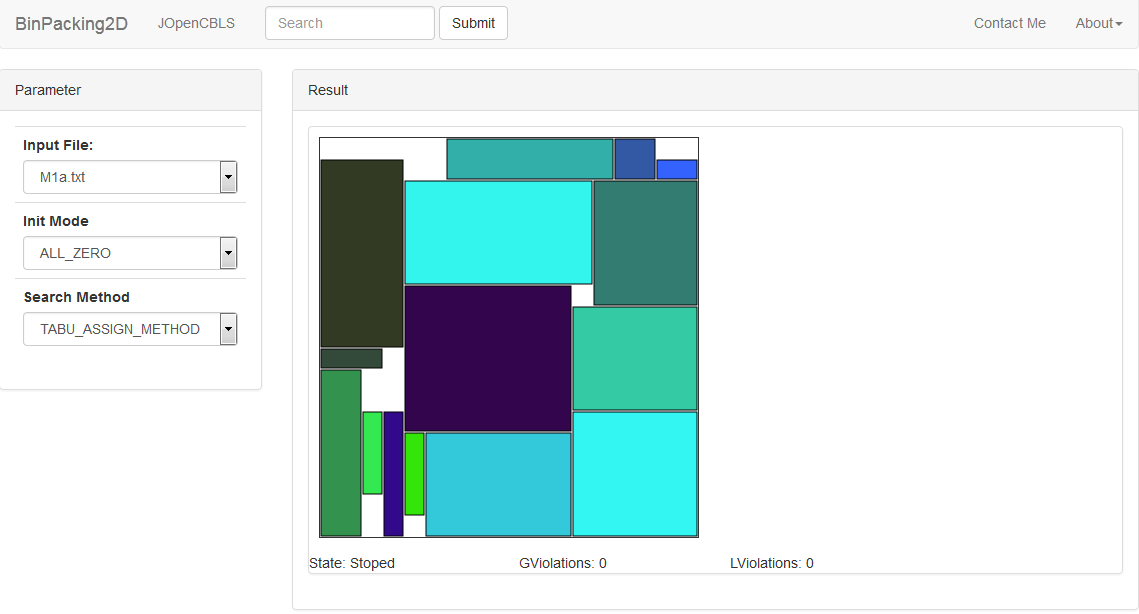
\includegraphics[scale=0.5]{figures/if-result.png}
	\caption{Giao diện kết quả chương trình \label{fig:ifResult}}
\end{figure}
Hình \ref{fig:ifResult} là giao diện sau khi thực hiện chương trình.
%==================================================================
\section{Kết quả thực nghiệm}
\subsection{Thực nghiệm}
Kết quả thực tế chạy trên các bộ dữ liệu mẫu được thống kê trong bảng \ref{tab:res}
{\scriptsize
\begin{table}[H]
	\centering
	\begin{threeparttable}
		%Thong ke thuat toan search asign
		\begin{tabular}{| l | c | c | c | c |}
			\hline
			\hline
			\multirow{ 2}{*}{Bộ DL\tnote{1}}
										& \multicolumn{2}{c}{RANDOM\tnote{2}} & \multicolumn{2}{c}{ALLZERO\tnote{2}} \\
			\cline{2-5}
										&Violations 		& Time(m)				& Violations		& Time (m)	\\
			\hline
			\hline

			M0a.txt 				 	&	0				&	1					& 	0			&	<1\\
			\hline
			M0b.txt 				 	&	0				&	10					& 	0			&	7\\
			\hline
			M1a.txt 				 	&	0				&	133					& 	0			&	19\\ 
			\hline
			M1b.txt 				 	&	0				&	243					& 	0			&	89\\ 
			\hline
			M1c.txt 					&	0				&	102					& 	0			&	267\\  
			\hline
			M1d.txt 					&	0				&	156					& 	0			&	78\\  
			\hline
			M1e.txt 					&	0\tnote{3}		&	378	    			& 	0\tnote{3}	&	326\\  
			\hline
			M1f.txt 					&	1				&	?					& 	1			&	?\\  
			\hline
			\hline
		\end{tabular}
		\begin{tablenotes}
			\item[1] Các bộ dữ liệu được cho trong \ref{tab:bpData}
			\item[2] Các số liệu được lấy từ giá trị trung bình 10 lần chạy trên mõi bộ dữ liệu bao gồm số bước lặp và thời gian thực thi.
			\item[3] Mục này chứa một vài lần thực thi cho kết quả vi phạm khác 0.
			\item[*] Kết quả thống kê được thực hiện trên máy tính intel với tốc độ xử lý 3.1GH với nền tảng Java 8.
		\end{tablenotes}
	\end{threeparttable}
    \caption{Kết quả thực thi trên các bộ dữ liệu mẫu của chương trình với thuật toán tìm kiếm Tabu cài đặt trong lớp \textsl{SearchTabuAssign} \label{tab:res}}

\end{table}
}

Các kết quả thống kê cho thấy bên cạnh thuật toán sẵn có trong thư viện JOpenCBLS thì các thuật toán cài đặt thêm đã cải thiện khá tốt khả năng tìm kiếm trong bài toán BP2D.

\subsection{Đánh giá chương trình}
\begin{itemize}
	\item \textbf{Ưu điểm}\\
	\begin{itemize}
		\item Giải quyết bài toán đóng thùng 2 chiều một cách có hiệu quả.
		\item Giao diện phầm mềm trực quan, dễ thao tác.
		\item Áp dụng nhiều công nghệ mới như AngularJS, Bootstrap, Java servlet, kiến trúc MVP để xây dựng chương trình.
		\item Sử dụng được tính mềm dẻo, tái sử dụng của thư viện JOpenCBLS.
	\end{itemize}
	\item \textbf{Nhược điểm}
	\begin{itemize}
		\item Chưa thực hiện và giải quyết trên bộ dữ liệu lớn.
	\end{itemize}
\end{itemize}